\documentclass[12pt,a4paper,titlepage]{scrartcl}

\usepackage{comment}
\usepackage[main=ngerman,english]{babel}
\usepackage[utf8]{inputenc}
\usepackage[T1]{fontenc}
\usepackage{lmodern}
\usepackage{geometry}
\geometry{left=2.5cm,right=2.5cm,top=2.5cm,bottom=3cm,head=29pt,foot=25pt}
\setlength{\footheight}{25pt}
\usepackage{microtype}
\usepackage{amsmath,amssymb,mathtools}
\numberwithin{equation}{section}
\numberwithin{table}{section}
\numberwithin{figure}{section}
\usepackage{siunitx}
\sisetup{locale=DE, separate-uncertainty=true, per-mode=fraction}
\usepackage{booktabs}
\usepackage{multirow}
\usepackage{graphicx}
\usepackage{float}
\usepackage{caption}
\usepackage{subcaption}
\usepackage[automark]{scrlayer-scrpage}
\usepackage[most]{tcolorbox}
\usepackage{hyperref}
\usepackage{pdfpages}
\usepackage{csvsimple-l3}
\usepackage{longtable}

%\input{../../jupyterpackages.tex}

% jupyter nbconvert --to latex 'Path'
% enferne usepackages und begin{document} und end{document}
% \input in main.tex mit \input{Path}


\newcommand{\pdfabbildung}[2]{%
    \refstepcounter{figure}%
    \addcontentsline{lof}{figure}{\protect\numberline{\thefigure}#1}%
    \label{#2}%
}

\newcommand{\pdftabelle}[2]{%
    \refstepcounter{table}%
    \addcontentsline{lot}{table}{\protect\numberline{\thetable}#1}%
    \label{#2}%
}


\hypersetup{colorlinks=true, linkcolor=blue!60!black, urlcolor=blue!60!black, citecolor=blue!60!black}

\clearpairofpagestyles

\chead{%
    \versuch\hfill\autor\\
    \rule{\textwidth}{0.2pt}%
}
\cfoot{%
    \rule{\textwidth}{0.2pt}\\[-0.5ex]
    \pagemark\ 
}
\addtokomafont{pagefoot}{\small}
\setlength{\parindent}{0pt}

\newtcolorbox{resultbox}[1][]{ 
    enhanced,
    colback=black!4!white,
    colframe=black!65!black,
    boxrule=0.8pt,
    arc=0.0mm,
    title=#1,
    fonttitle=\bfseries,
    %drop shadow
}


\newcommand{\versuch}{Versuch 33}
\newcommand{\titel}{Prismenspekrometer}
\newcommand{\praktikum}{Physikalisches Anfängerpraktikum 1}
\newcommand{\autor}{Jonathan Gießen}
\newcommand{\gruppe}{Gruppe 8}
\newcommand{\datum}{10. September 2026}
\newcommand{\betreuer}{Sebastian Hurth}

\begin{document}

\pagestyle{scrheadings}

\begin{titlepage}



    \centering
    \vspace*{4cm}
    {\large Universität Heidelberg\par}
    {\small Fakultät für Physik und Astronomie\par}
    {\Large \praktikum\par}
    \vspace{0.8cm}
    {\LARGE \bfseries \versuch\ -- \titel\par}
    \vspace{1.5cm}

    \begin{tabular}{ll}
        \textbf{Autor:} & \autor\\
        \textbf{Gruppe:} & \gruppe\\
        \textbf{Betreuer:} & \betreuer\\
        \textbf{Versuchsdatum:} & \datum\\
    \end{tabular}

    \vfill
    \hrulefill\
\end{titlepage}

\tableofcontents

\bigskip
\begin{tcolorbox}[colback=gray!5,colframe=gray!60,boxrule=0.8pt,arc=0.01mm,title=KI-Hinweis]
    Für die sprachliche Formulierung dieses Protokolls wurde in der Einleitung \ref{sec:Einleitung} KI-gestützte Textgenerierung verwendet.
\end{tcolorbox}

\clearpage
\section{Einleitung}\label{sec:Einleitung}
Der Versuch 33 mit der Funktionsweise und Anwendung eines Prismenspektrometers. Hauptziel des Versuches ist es, die spektrale Zerlegung von Licht durch die Dispersion an einem optischen Prisma quantitativ zu untersuchen. 

Dazu wird zunächst die Winkeldispersionskurve $\delta(\lambda)$ des Prismas unter Ausnutzung des Minimalablenkwinkels aufgenommen, indem die bekannten Spektrallinien einer Quecksilberdampflampe vermessen werden. Diese Eichkurve dient im Anschluss dazu, die unbekannten Emissionswellenlängen eines Heliumspektrums präzise zu bestimmen. 

Ergänzend bietet der Versuch weiterführende spektroskopische Analysen: Durch die Vermessung der sichtbaren Balmer-Serie im Wasserstoffspektrum kann die Rydberg-Konstante experimentell abgeleitet werden. Das experimentelle Verständnis dieser optischen und quantenmechanischen Effekte bildet eine essenzielle Basis für die Spektroskopie in der Experimentalphysik.


\section{Grundlagen und Theorie}
Das verwendete Prisemspekrometer basiert darauf, dass Licht unterschiedlicher Wellenlängen beim Durchgang durch ein optisches Prisma unterschiedlich stark gebrochen wird. Dies führt zu einer spektralen Zerlegung des Lichts, die als Dispersion bezeichnet wird. abei handelt es sich um einen Körper aus einem lichtdurchlässigen Material, (hier Glas) der von zwei ebenen, nicht parallelen Flächen begrenzt wird. Die Gerade, in der sich die beiden Flächen schneiden, wird brechende Kante genannt. In einem Schnitt senkrecht dazu (Hauptschnitt) liegt an der brechenden Kante der brechende Winkel $\varepsilon$.\cite{PAPskript}: 
\begin{figure}[H]
    \centering
    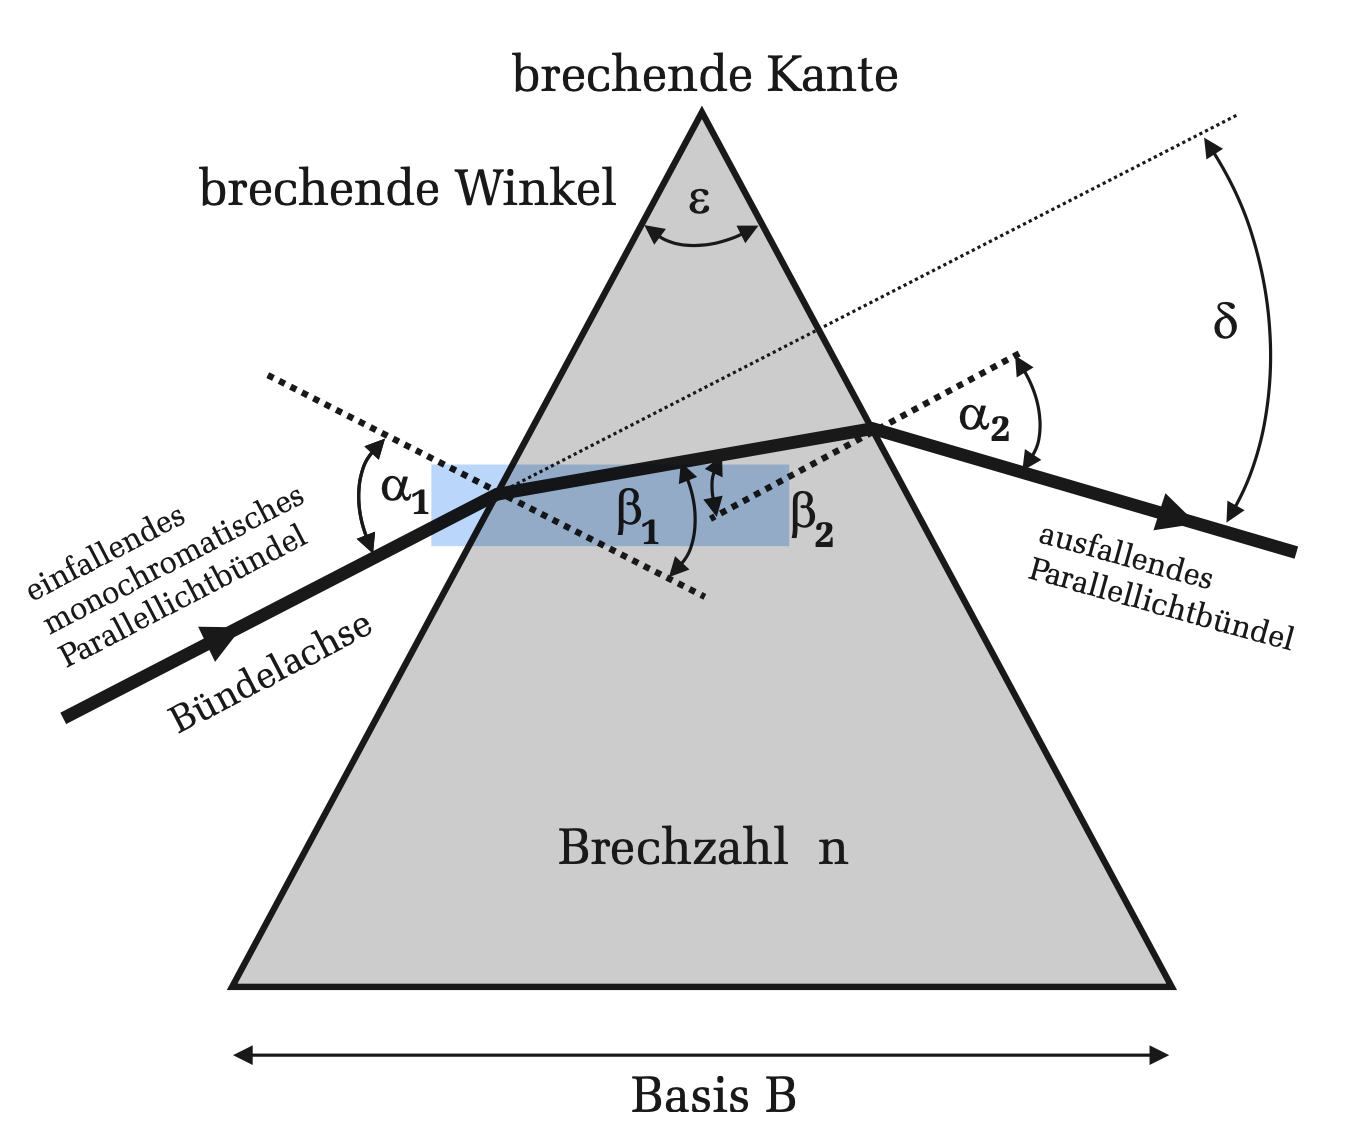
\includegraphics[width=0.5\textwidth]{img/Prismenspektrometer.png}
    \caption{Schematische Darstellung eines Prismenspektrometers.}
    \label{fig:Prismenspektrometer}
\end{figure}

Mit Hilfe des Brechungsgesetzes und unter der Annahme, dass für den Brechungsindex von Luft $n_\text{luft} = 1$ gilt, folgt für den totalen Ablenkungswinkel $\delta$, um den ein einfallendes Lichbündel abgelenkt wird:

\begin{equation}
    \delta = \alpha_1 - \varepsilon + \arcsin\left(\sqrt{n^2 - \sin(\alpha_1)^2}\sin(\varepsilon)-\sin(\alpha_1)\cos(\varepsilon)\right)\label{eq:total_angle}
\end{equation}

Aufgrund von Dispersion ist der Brechungsindex $n$ des Prismas eine Funktion der Wellenlänge $\lambda$ des Lichts. Somit folgt mit $n(\lambda)$
\begin{equation}
    \delta(\lambda) = \alpha_1 - \varepsilon + \arcsin\left(\sqrt{(n(\lambda))^2 - \sin(\alpha_1)^2}\sin(\varepsilon)-\sin(\alpha_1)\cos(\varepsilon)\right)\label{eq:total_angle_lambda}
\end{equation}

Um nun das Emissionsspektrum einer Lichtquelle zu bestimmen wird zunächst die Winkeldispersionskurve $\delta(\lambda)$ des Prismas aufgenommen, indem die bekannten Spektrallinien einer Quecksilberdampflampe vermessen werden. Diese Eichkurve dient im Anschluss dazu, die unbekannten Emissionswellenlängen eines Heliumspektrums präzise zu bestimmen. Im Rahmen des Versuches wird zudem die Rydberg-Konstante experimentell abgeleitet, indem die sichtbare Balmer-Serie im Wasserstoffspektrum vermessen wird. Das experimentelle Verständnis dieser optischen und quantenmechanischen Effekte bildet eine essenzielle Basis für die Spektroskopie in der Experimentalphysik.


\section{Messprotokoll und Durchführung}

\subsection{Durchführung}

\paragraph{Justage des Spektrometers}
Zu Beginn des Versuchs wurde das Prismenspektrometer justiert. Das Fernrohr wurde auf ein weit entferntes Objekt (unendlich) gerichtet und das Fadenkreuz im Okular parallaxenfrei scharfgestellt. Anschließend wurde der Spalt des Kollimators mit einer Quecksilberdampflampe (Hg) beleuchtet und das Kollimatorrohr verschoben, bis im justierten Fernrohr ein scharfes Spaltbild zu beobachten war, um sicherzugehen. dass es sich um parallele Strahlen .

\paragraph{Aufgabe 1: Aufnahme der Eichkurve (Hg-Spektrum)}
Das Prisma wurde auf den Prismentisch gesetzt. Durch Drehen des Tisches wurde der Minimalablenkwinkel für die starke grüne Hg-Linie gesucht und eingestellt. In dieser fixierten Prismenposition wurden anschließend die Ablenkwinkel $\delta$ für zehn vorgegebene Linien des Quecksilberspektrums einseitig vermessen. Für eine hohe Präzision wurde die Teilkreisskala in Kombination mit dem Nonius verwendet.

\paragraph{Aufgabe 2: Bestimmung des He-Spektrums}
Unter strikter Beibehaltung der zuvor gewählten Prismen- und Skaleneinstellung (Minimalablenkung für die grüne Hg-Linie) wurde die Lichtquelle gewechselt. Die Ablenkwinkel von sechs sichtbaren Linien einer Heliumlampe (He) wurden abgelesen.

\paragraph{Zusatzaufgabe 1: Balmer-Serie des Wasserstoffspektrums}
Zuletzt wurde das Spektrometer mit einer Wasserstofflampe beleuchtet. Bei unveränderter Geräteeinstellung wurden die Ablenkwinkel der drei stärksten sichtbaren Spektrallinien (rot, türkis, violett) sowie einer vierten, schwächeren Linie abgelesen.

\subsection{Messprotokoll}
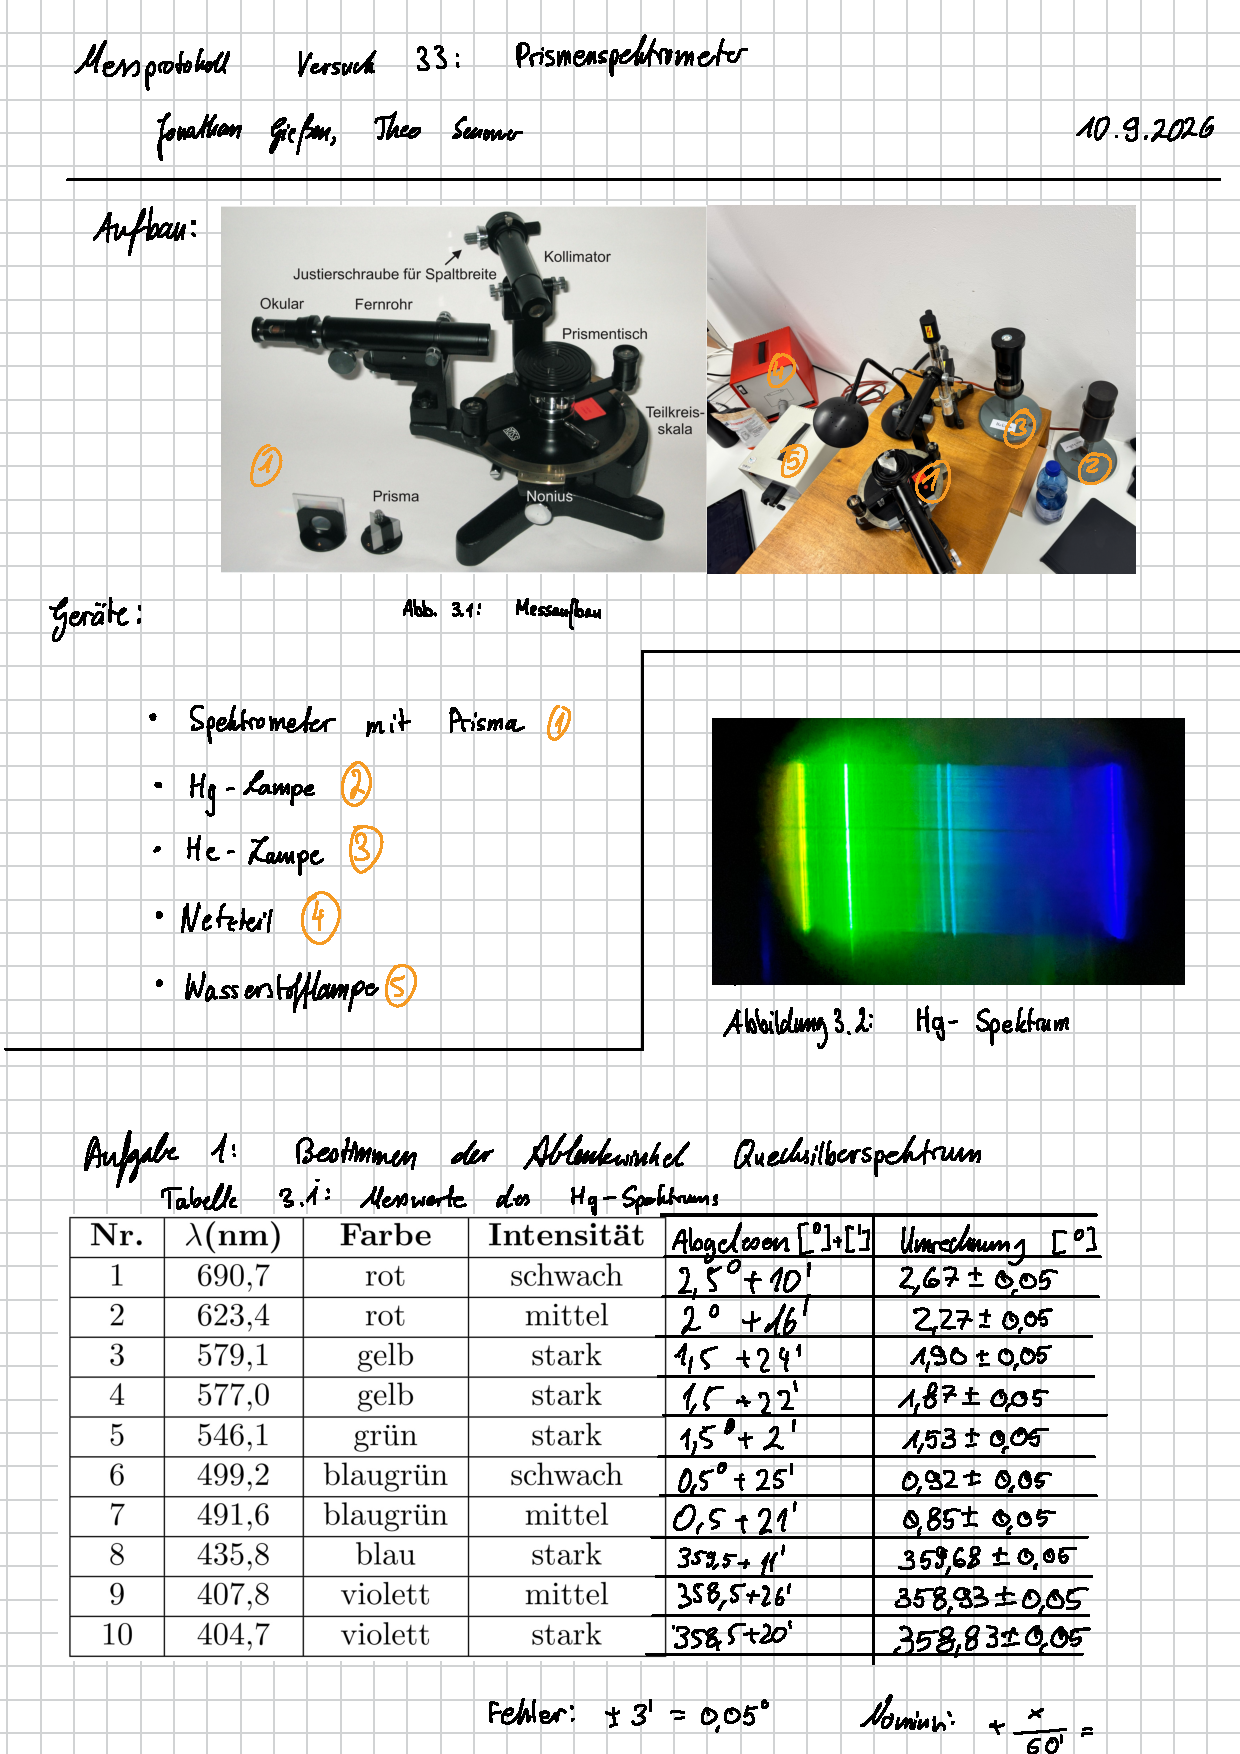
\includepdf[
    pages=-,
    width=\textwidth,
    height=\textheight,
    keepaspectratio,
    pagecommand={\thispagestyle{scrheadings}}
]{../Messprotokoll 33.pdf}


\pdfabbildung{Messaufbau}{fig:pdf-1}
\pdfabbildung{Hg-Spektrum}{fig:pdf-2}
\pdfabbildung{He-Spektrum}{fig:pdf-3}
\pdfabbildung{Wasserstoff-Spektrum}{fig:pdf-4}
\pdfabbildung{Epischer Messaufbau}{fig:pdf-5}

\pdftabelle{Ablenkwinkel des Quecksilber-Spektrums}{tbl: Messwerte_Hg}
\pdftabelle{Ablenkwinkel des Helium-Spektrums}{tbl: Messwerte_He}
\pdftabelle{Ablenkwinkel des Wasserstoff-Spektrums}{tbl: Messwerte_H}

\section{Auswertung}

\subsection{Aufgabe 1: Zeichnen der Eichkurve mit den bekannten Spektrallinien des Quecksilberspektrums}





\clearpage

\listoffigures


\listoftables

\begin{thebibliography}{5}
    \bibitem{PAPskript} Dr. J.Wagner, \emph{Physikalisches Anfängerpraktikum}, Stand 11/2024
    \bibitem{ilberg1988physikalisches} W. Ilberg, M. Krötzsch, \emph{Physikalisches Praktikum für Anfänger}, BSB B. G. Teubner Verlagsgesellschaft, Leipzig (1985).
\end{thebibliography}




\begin{comment}

\begin{table}[H]
    \centering
    \caption{Mess- und Geräteparameter für die exemplarische Berechnung (Messung 28).}
    \label{tab:parameter_messung_28}
    \begin{tabular}{ll}
        \toprule
        \textbf{Größe} & \textbf{Wert} \\
        \midrule
        Fallstrecke & $s_1 = 10\,\text{Skt} = 5.00 \cdot 10^{-4}\,\text{m}$ \\
        Fallzeit & $t_1 = 11.85\,\text{s}$ \\
        Steigstrecke & $s_2 = 10\,\text{Skt} = 5.00 \cdot 10^{-4}\,\text{m}$ \\
        Steigzeit & $t_2 = 18.19\,\text{s}$ \\
        Skalenteilung & $1\,\text{Skt} = 5.00 \cdot 10^{-5}\,\text{m}$ \\
        Kondensatorspannung & $U = 500\,\text{V}$ \\
        Plattenabstand & $d = 6.00 \cdot 10^{-3}\,\text{m}$ \\
        Luftdruck & $p = 100285\,\text{Pa}$ \\
        Erdbeschleunigung & $g = 9.81\,\frac{\text{m}}{\text{s}^2}$ \\
        Dichtedifferenz & $\rho = \rho_{\text{Öl}} - \rho_{\text{Luft}} = 871.21\,\frac{\text{kg}}{\text{m}^3}$ \\
        Unkorrigierte Luftviskosität & $\eta_0 = 1.81 \cdot 10^{-5}\,\text{Pa}\cdot\text{s}$ \\
        Cunningham-Konstante & $b = 7.78 \cdot 10^{-3}\,\text{Pa}\cdot\text{m}$ \\
        \bottomrule
    \end{tabular}
\end{table}
\end{comment}
\end{document}